\documentclass[12pt]{beamer}
\usepackage[english, russian]{babel}
\usepackage[utf8x]{inputenc}
\usepackage{itmobeamer}
\usepackage{makecell}
\usepackage{tabularx}
\usepackage{multicol}
\usepackage{caption}
\usepackage{listings}
\usepackage{subcaption}

\lstset{emph={
    tc, qdisc, class, dev, parent, classid, filter, protocol, flowid, cbwfq, default, bandwidth,
    },emphstyle={\bfseries}%
}%

\title[Реализация CBWFQ в ядре Linux]{Реализация дисциплины обслуживания CBWFQ для ядра Linux}
\author[]{{\small Автор: Куклина Мария Дмитриевна\\ Научный руководитель: Шинкарук Дмитрий Николаевич}}
\institute[]{Университет ИТМО}
\date[]{Санкт-Петербург, 2018}

\setbeamertemplate{caption}[numbered]

\begin{document}

\setcounter{figure}{0}

\newcommand{\mc}[0]{\makecell}
\newcommand\setrow[1]{\gdef\rowmac{#1}#1\ignorespaces}
\newcommand\clearrow{\global\let\rowmac\relax}
\clearrow
%\itmologoslide

\begin{darkbars}
    \begin{frame}[noheader,nologo,noframenumbering]
        \titlepage
    \end{frame}
\end{darkbars}

\begin{frame}{Цели и задачи}
    \textbf{Цель} -- реализация дисциплины обслуживания Class-Based Weighted Fair Queueing
    (CBWFQ) в ядре Linux. \newline

    \textbf{Задачи}
    {\small
        \begin{itemize}

    \item Проанализировать и сравнить дисциплины обслуживания PQ, CBQ, HTB, HFSC, FWFQ, CBWFQ.
    \item Восстановить алгоритмы Class-Based WFQ.
    \item Настроить среду для реализации и тестирования.
    \item Реализовать модуль ядра CBWFQ в ядре Linux.
    \item Реализовать интерфейс утилиты tc для управления модулем.
    \item Провести тестирование.
        \end{itemize}
    }
\end{frame}

\begin{frame}{Weighted Fair Queueing}
	
	\textbf{General Processor Sharing (GPS)} -- математическая модель
	планировщика, позволяющая максимально точно разделить пропускную
	способность между классами трафика в соответствии с назначенными
	весами.

	\textbf{WFQ} -- взвешенный алгоритм честного обслуживания,
	представляющий собой аппрокисмацию модели GPS; он оперирует
	пакетами, предоставляя максимально честное обслуживание,
	которое возвомжно для данного алгоритма при работе с пакетами.

\end{frame}


\begin{frame}{WFQ на основе вычисления порядкового номера пакета}
	\begin{figure}
		\center
    	\includegraphics[scale=0.7]{../text/pdfimages/wfq_seq.pdf}
		\caption{Схема обслуживания пакетов в WFQ}
	\end{figure}
	
	Порядковый номер пакета вычисляется на основе длины пакета, веса потока и
	текущего счётчика циклов (или порядкового номера последнего обслуженного пакета в потоке).

	%{\scriptsize
	%CDT (congestive discard threshold) -- количество пакетов в системе WFQ перед началом отбрасывания.\\
	%HQO (hold queue out) -- максимальное количество пакетов во всех выходящих очередях.
	%}
\end{frame}


\begin{frame}{Flow-based Weighted Fair Queueing}
	\begin{figure}
		\center
    	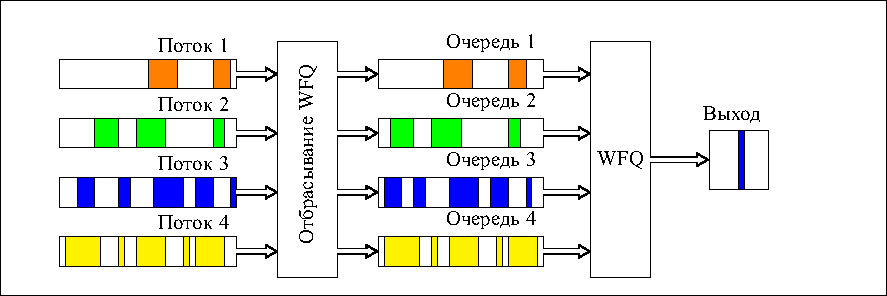
\includegraphics[scale=0.6]{../text/pdfimages/fwfq.pdf}
		\caption{Схема движения пакетов в планировщике FWFQ}
	\end{figure}
	\begin{center}
        {\footnotesize
            \begin{multicols}{2}
				{\bf Преимущества}
				\begin{itemize}
					\item Простая конфигурация.
					\item Отбрасывание пакетов из агрессивных потоков.
					\item Честное обслуживание.
				\end{itemize}
            \columnbreak
				{\bf Недостатки}
				\begin{itemize}
					\item Нельзя разделять трафик по классам обслуживания.
					\item Не предоставляет задание определённой пропускной способности.
				\end{itemize}
            \end{multicols}
		}
	\end{center}
\end{frame}



\begin{frame}{Class-Based Weighted Fair Queueing}
	\begin{figure}
		\center
    	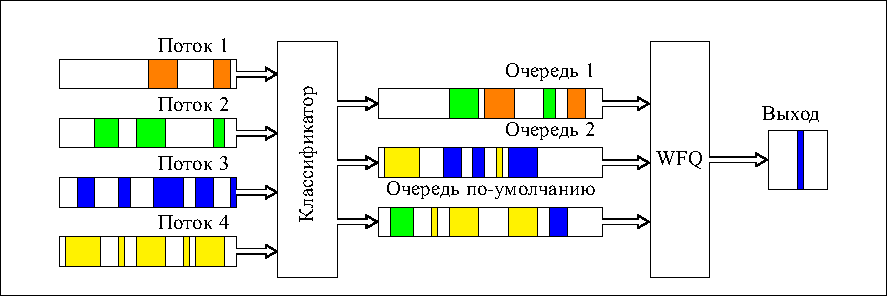
\includegraphics[scale=0.7]{../text/pdfimages/cbwfq.pdf}
		\caption{Схема движения пакетов в планировщике CBWFQ}
	\end{figure}

	\begin{center}
{\footnotesize
            \begin{multicols}{2}
				{\bf Преимущества}
				\begin{itemize}
					\item Гибкая конфигурация классов.
					\item Выделение заданной пропускной способности для классов.
				\end{itemize}
            \columnbreak
				{\bf Недостатки}
				\begin{itemize}
					\item Ограничение на количество пользовательских классов.
					\item Плохо работает с интерактивным трафиком.
				\end{itemize}
            \end{multicols}
}
	\end{center}
\end{frame}

\begin{frame}{Сравнительная таблица ДО}
%{\footnotesize
%    \begin{tabular}{|>{\rowmac}c|>{\rowmac}c|>{\rowmac}c|>{\rowmac}c|>{\rowmac}c|>{\rowmac}c|>{\rowmac}c<{\clearrow}|}
%        \hline
%\setrow{\bfseries}               Свойство     & PQ   & CBQ   & HTB   & HFSC  & FWFQ  & CBWFQ \\ \hline
%{\bf \mc{Метод\\ планирования}   }& RR   &WRR    & RR    & RT/LS & WFQ   & WFQ   \\ \hline
%{\bf Честность                   }& -    & -     & -     & +     &  +    &  +    \\ \hline
%{\bf      Отбрасывание           }&{\scriptsize  TD   }&{\scriptsize  TD    }&{\scriptsize  TD    }&{\scriptsize  TD    }&{\scriptsize  ED/AD }&{\scriptsize  TD/WRED }\\ \hline
%{\bf \mc{Разделение\\ канала}    }& -    &  +    &  +    &  +    &  -    &  -    \\ \hline
%{\bf \mc{Сложность \\ реализации}}& {\scriptsize Низкая }& {\scriptsize Высокая     }&  {\scriptsize Средняя    }&  {\scriptsize Высокая    }&   {\scriptsize Средняя   }&  {\scriptsize Средняя}\\ \hline
%{\bf \mc{Конфигурация\\ классов}}		  & -  & + & + & + & - & + \\ \hline
%{\bf \mc{Реализация\\ в Linux}}   & + & + & + & + & - & -  \\ \hline
%    \end{tabular}
%}

{\scriptsize
        \begin{tabular}{|>{\rowmac}c|>{\rowmac}c|>{\rowmac}c|>{\rowmac}c|>{\rowmac}c|>{\rowmac}c|>{\rowmac}c<{\clearrow}|}
            \hline
            \setrow{\bfseries}     Свойство        & PQ   & CBQ   & HTB   & HFSC  & FWFQ  & CBWFQ \\ \hline
            {\bf \mc{Метод\\ планирования        }}& RR   & WRR   & RR    & RT/LS & WFQ   & WFQ   \\ \hline
            {\bf Отбрасывание                     }& TD   & TD    & TD    & TD    & ED/AD & TD/WRED \\ \hline
            {\bf \mc{Честность\\(справедливость) }}& -    & -     & -     & -     &  +    &  +    \\ \hline
            {\bf \mc{Разделение\\ канала         }}& -    &  +    &  +    &  +    &  -    &  -    \\ \hline
			{\bf \mc{Решение проблемы\\ голодания}}& -    &  +    & +     & +     & +     & +    \\ \hline
            {\bf \mc{Сложность \\ реализации     }}& Низк & Выс   &Сред   & Выс   & Сред  & Сред \\ \hline
            {\bf \mc{Сложность \\ конфигурации   }}& Низк & Выс   &Сред   & Выс   & Низк  & Низк \\ \hline
            {\bf \mc{Конфигурация\\ классов      }}& -    & +     & +     & +     & -     & + \\ \hline
            {\bf \mc{Реализация\\ в Linux        }}& +    & +     & +     & +     & -     & -  \\ \hline
        \end{tabular}
}
{\scriptsize
	Обозначения:
	 RR -- Round Robin, RT/LS -- на основе Real Time/Link Sharing критериев.\\
	 TD -- Tail Drop, ED -- Early Dropping, AD -- Aggressive Dropping.
}
\end{frame}


\begin{frame}{Дисциплины обслуживания}
	% TODO: сделать рисунок более понятным
	\textbf{Дисциплина обслуживания (qdisc, ДО)} -- набор алгоритмов,
	определяющий метод организации очереди, способы выбора пакета из очереди,
	политику отбрасывания пакетов и способы выделения канала.
	\begin{figure}
		\center
    	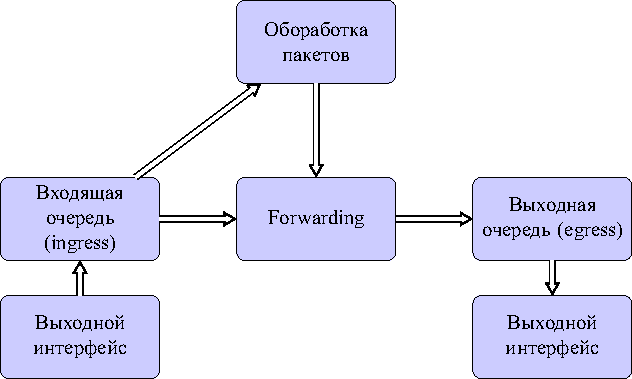
\includegraphics[scale=0.7]{../text/pdfimages/qdisc.pdf}
	\end{figure}


\end{frame}

\begin{frame}[fragile]{Тестирование модуля}
	\begin{figure}
		\center
    	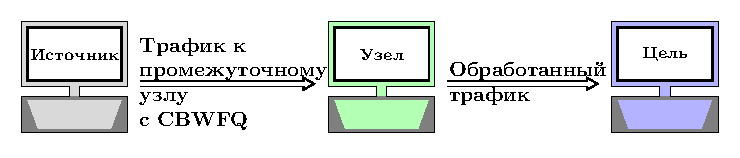
\includegraphics[scale=0.7]{../text/pdfimages/test_scheme.pdf}
		\caption*{{\footnotesize Схема тестовой среды}}
	\end{figure}
{\footnotesize
	\begin{lstlisting}[frame=single]
tc qdisc add dev eth1 cbwfq bandwidth 100Mpbs \
 default rate 30 percent
tc class add dev eth1 parent 1: classid 1:3 \
 cbwfq rate 70 percent  
tc filter add dev ens3 parent 1: protocol ip \
 u32 match ip sport $TESTPORT1 flowid 1:2

    \end{lstlisting}
}
\end{frame}

\begin{frame}{Тестирование модуля}
	\begin{figure}
		\center
    	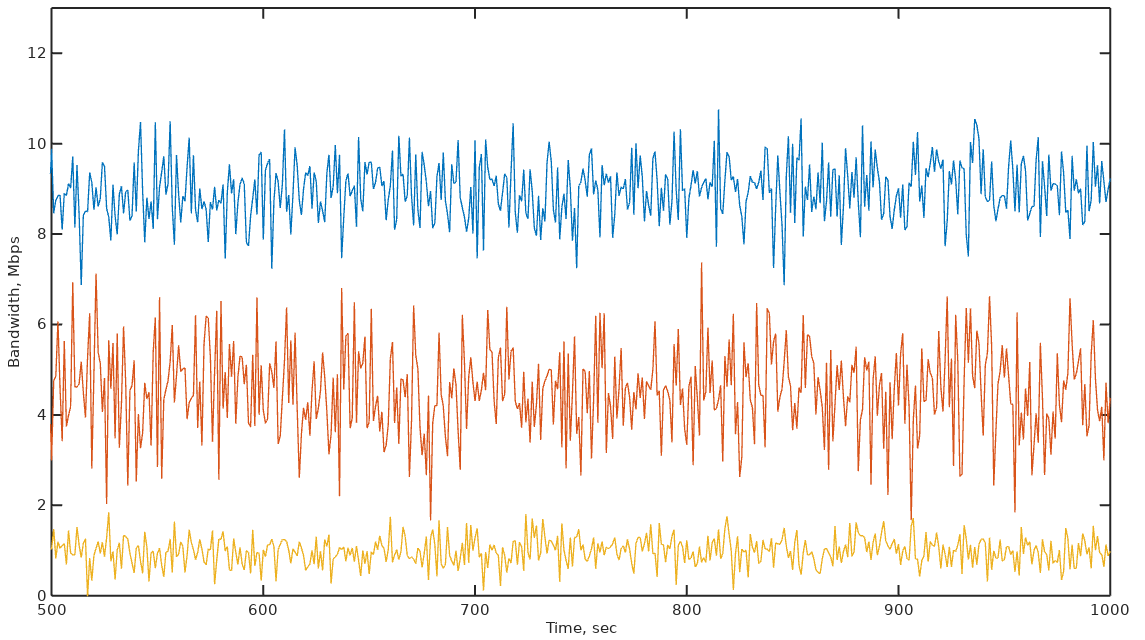
\includegraphics[scale=0.4]{../text/pdfimages/plot.pdf}
		\caption{{\scriptsize График распределения доли пропускной способности в течение времени.}}
	\end{figure}
\end{frame}

\begin{frame}{Вывод}
	\begin{itemize}
		\item Проведён сравнительный анализ классовых дисциплин обслуживания.
		\item Проведено исследование модели WFQ.
		\item Реализован интерфейс для системы tc.
		\item Реализован алгоритм CBWFQ в ядре Linux.
		\item Перспектива развития работы: реализация алгоритма WRED и доработка модуля до дисциплины LLQ.
	\end{itemize}
\end{frame}

\itmothankyou

\end{document}
